%\chapter{Main Results}
\chapter{実験と考察}

\section{実験環境,前提}

実験環境として,2次元の有限な擬似連続空間とし,被動作対象であるトラジェクタ(赤)と,参照点となりうる4つの物体(青,橙,緑,黄)が存在する空間内での物体移動動作の学習と再現,識別を行うシミュレータ環境を準備した.被教示者にとって,空間の範囲,トラジェクタや物体の数,位置,観点の種類は既知で教示者と認識を共有しており,各動作における観点については未知であるとし,その観点を教示動作から獲得し,動作の再現と識別を行うことを目標とする.
%%%%%%%%%%%%%%%%%%%%%%%%%%%%%%%%%%%%%%%%%%%%%%%%%%%%%%%%%%%%%%%%%%%%%%%%%%%%%%%%%%%%%%%%%%%%%%%%%%%%%%%
	\begin{figure}[b]
%中央ぞろえ
		\begin{center}
			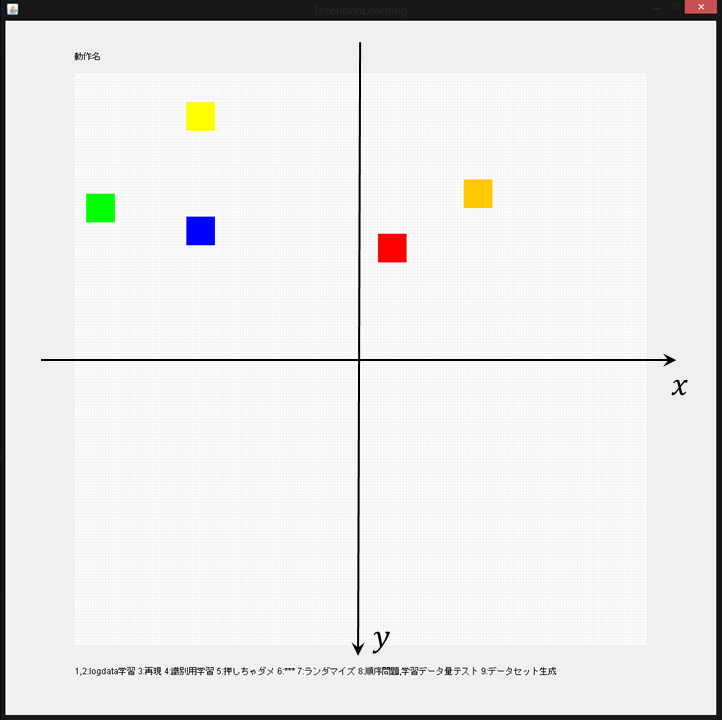
\includegraphics[width=8cm]{figure3.png} \\ %TeXの基本として, \\ で緊急改行ができる.(今回の場合や行列などを除き,あまり使わない)
			\caption{シミュレータ}
		\end{center}
	\end{figure}
%%%%%%%%%%%%%%%%%%%%%%%%%%%%%%%%%%%%%%%%%%%%%%%%%%%%%%%%%%%%%%%%%%%%%%%%%%%%%%%%%%%%%%%%%%%%%%%%%%%%%%%

\begin{table}[h]
	\caption{動作名とトラジェクタ目標位置の対応表}
	\label{table:taskname_15}
  	\begin{tabular}{|l|l|} \hline
    	動作名 & トラジェクタ目標位置\\ \hline
   	$T_{1}$ : 赤を中央に移動する & 
	$
    	\left( x_{center} , y_{center} \right)+G_{error}
    	$
    	\\
    	$T_{2}$ : 赤を青の右に移動する & 
	$
    	\left( x_{blue}+15 , y_{blue} \right)+G_{error}
    	$
%    	\\
%    	$T_{3}$ : 赤を橙の右に移動する & 
%	$
%    	\left( x_{orange}+15 , y_{orange} \right)+G_{error}
%    	$
%    	\\
%    	$T_{4}$ : 赤を緑の右に移動する & 
%	$
%    	\left( x_{green}+15 , y_{green} \right)+G_{error}
%    	$
%    	\\
%    	$T_{5}$ : 赤を黄の右に移動する & 
%	$
%    	\left( x_{yellow}+15 , y_{yellow} \right)+G_{error}
%    	$
%    	\\
%    	$T_{6}$ : 赤を青に近づける & 
%	$
%    	\left( \frac{x_{red}+x_{blue}}{2} , \frac{y_{red}+y_{blue}}{2} \right)+G_{error}
%    	$
    	\\
    	$T_{3}$ : 赤を橙に近づける & 
	$
    	\left( \frac{x_{red}+x_{orange}}{2} , \frac{y_{red}+y_{orange}}{2} \right)+G_{error}
    	$
%   	\\
%   	$T_{8}$ : 赤を緑に近づける & 
%	$
%    	\left( \frac{x_{red}+x_{green}}{2} , \frac{y_{red}+y_{green}}{2} \right)+G_{error}
%    	$
%    	\\
%    	$T_{9}$ : 赤を黄に近づける & 
%	$
%    	\left( \frac{x_{red}+x_{yellow}}{2} , \frac{y_{red}+y_{yellow}}{2} \right)+G_{error}
%    	$
%    	\\
%    	$T_{10}$ : 赤を青から遠ざける & 
%	$
%    	\left( 2x_{red}-x_{blue} , 2y_{red}-y_{blue} \right)+G_{error}
%    	$
%    	\\
%    	$T_{11}$ : 赤を橙から遠ざける & 
%	$
%    	\left( 2x_{red}-x_{orange} , 2y_{red}-y_{orange} \right)+G_{error}
%    	$
    	\\
    	$T_{4}$ : 赤を緑から遠ざける & 
	$
    	\left( 2x_{red}-x_{green} , 2y_{red}-y_{green} \right)+G_{error}
    	$
%    	\\
%    	$T_{13}$ : 赤を黄から遠ざける & 
%	$
%    	\left( 2x_{red}-x_{yellow} , 2y_{red}-y_{yellow} \right)+G_{error}
%    	$
    	\\
    	$T_{5}$ : 等間隔に赤,黄,青と並べる & 
	$
    	\left( 2x_{yellow}-x_{blue} , 2y_{yellow}-y_{blue} \right)+G_{error}
    	$
    	\\
    	$T_{6}$ : 時計回りに赤,緑,青と並べる & 
	$
	\begin{pmatrix}
        	\cos \frac{\pi}{3} & -\sin \frac{\pi}{3} \\
        	\sin \frac{\pi}{3} & \cos \frac{\pi}{3}
	\end{pmatrix}
	\begin{pmatrix}
        	x_{blue}-x_{green} \\
        	y_{blue}-y_{green}
	\end{pmatrix}
      	+
	\begin{pmatrix}
        	x_{green} \\
        	y_{green}
	\end{pmatrix}      	
	+G_{error}
    	$
    	\\ \hline
  	\end{tabular}
\end{table}
また本実験において使用した動作の,動作名とその動作におけるトラジェクタの目標位置をまとめた表をTable \ref{table:taskname_15}に示す.
ただし,Table \ref{table:taskname_15}における$x , y$は各物体の,画面中央を原点とし,画面に水平な$x$座標と,画面に垂直な$y$座標を規定した座標系(以下,画面座標)における座標成分である.また全ての物体は1辺が画面座標における10マス分の正方形とし,空間の範囲は画面座標における$x,y$軸ともに[-200 , 200]とした.$G_{error}$とは平均0のガウス分布から生起される誤差(以下,ガウス誤差)であり,分散の大きさは各実験ごとに設定する.$G_{error}$は教示誤差を表し,分散が小さいほど正確に与えられた教示動作となる.


\section{動作再現}

提案手法によって動作の学習が適切に行えていることを確認するため,
観点が被教示者にとって未知である教示動作を与え,観点を推定し動作を再現する実験を行った.
動作再現の実験にはTable \ref{table:taskname_15}の6動作を使用した.

\subsection{教示誤差と再現誤差の関係に関する実験}

動作教示時に生じた誤差(教示誤差)が,動作再現時に生じる誤差(再現誤差)にどのように影響するか調べるために,教示誤差を変化させながら再現誤差を計測する実験を行った.
教示誤差をガウス誤差の分散0.5間隔で0から20まで増やしながらそれぞれ500データ生成し,10データ1セットの一つ抜き法で再現誤差の計算を各教示誤差で計50回ずつ行った.
観点推定の成否の判定は計算結果のうち各教示誤差における標準偏差の2.896倍\footnote{付録\ref{appendix2}参照}以上の誤差が生じた再現結果を推定失敗と定めた.Fig.\ref{figure:success_rate}に,そのようにして各再現結果を成功と失敗に分けた観点推定の正答率のグラフを示す.なお,正答率の計算に用いた実験結果については付録\ref{appendix1}に示す.また付録\ref{appendix2}に,各教示誤差と再現誤差の関係と,判定基準を上記のように定められることの詳細を示す.
%%%%%%%%%%%%%%%%%%%%%%%%%%%%%%%%%%%%%%%%%%%%%%%%%%%%%%%%%%%%%%%%%%%%%%%%%%%%%%%%%%%%%%%%%%%%%%%%%%%%%%%
	\begin{figure}[h]
%中央ぞろえ
		\begin{center}
			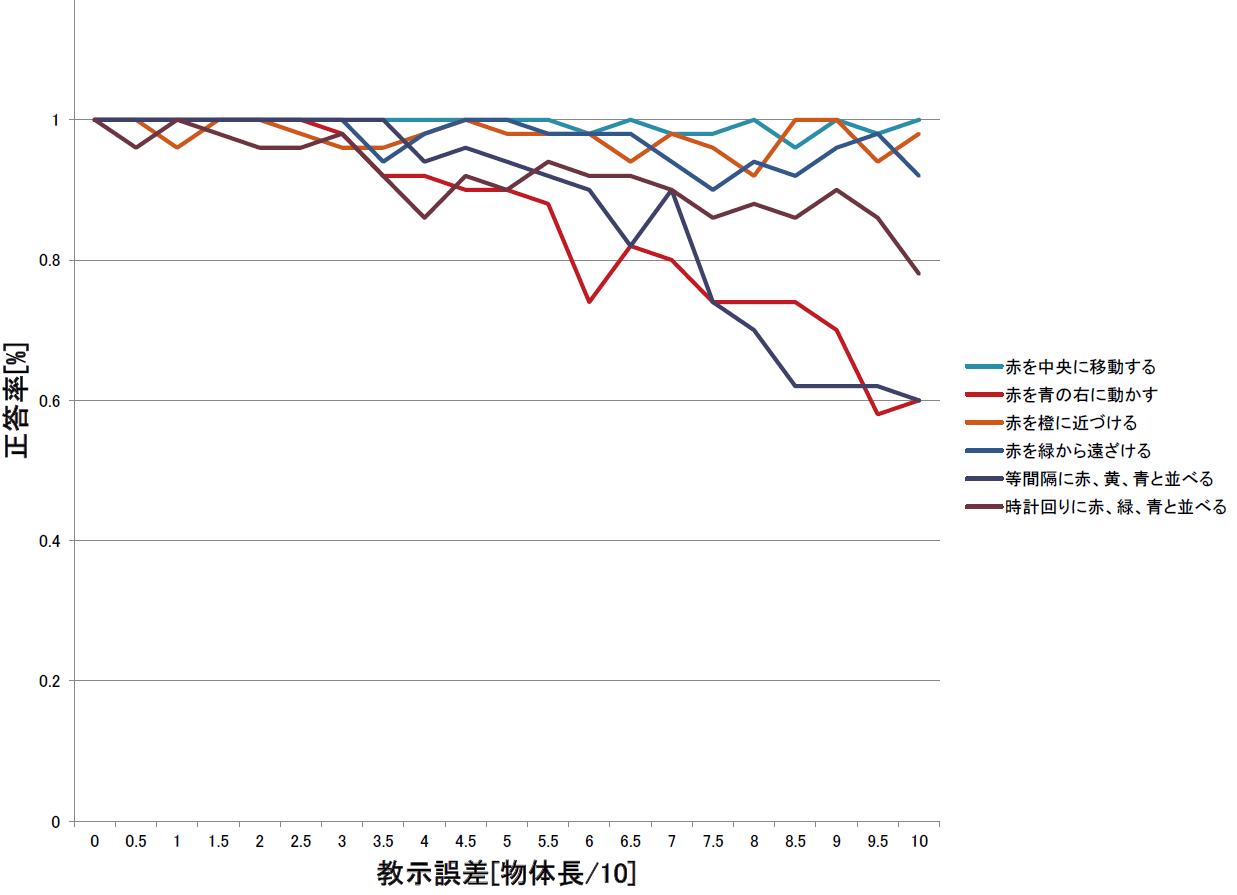
\includegraphics[width=14cm]{chart2.png} \\ %TeXの基本として, \\ で緊急改行ができる.(今回の場合や行列などを除き,あまり使わない)
			\caption{教示誤差と正答率の関係のグラフ}
			\label{figure:success_rate}
		\end{center}
	\end{figure}
%%%%%%%%%%%%%%%%%%%%%%%%%%%%%%%%%%%%%%%%%%%%%%%%%%%%%%%%%%%%%%%%%%%%%%%%%%%%%%%%%%%%%%%%%%%%%%%%%%%%%%%

Fig.\ref{figure:success_rate}から,教示誤差が十分に小さい場合に,観点の推定が適切に行えていることがわかる.また,$T_{5}$,$T_{6}$においても十分に正確な教示動作において適切に再現できていることから,複数の参照点を含む動作を適切に学習できていることがわかる.実験に使用した動作のうち,$T_{1}$,$T_{3}$,$T_{4}$の正答率が意図した状態と異なり,教示誤差の増加に無関係に再現できているが,これは学習時の遷移ベクトルの正規化関数における正規化長に依るものだと考えられる.また中央に移動する動作は中央に近づける動作とも認識できる等,適切な観点が複数存在する動作に関して誤答率が下がったとも考えられる.

\subsection{正規化長に関する考察}
\label{subsection:UNIT}
動作学習時に教示動作に適応される正規化関数$Normalize_{lk}(v)$は\ref{equation:normalize}式で表される.ここで,$unit$は正規化長を表す.正規化関数は,教示動作から得られた参照点から目標位置までの相対位置ベクトルを,あらかじめ定めた正規化長に正規化する.これは例えば物体に近づける動作など,距離的な位置関係よりも初期位置からの変化の割合が重視されるような動作や,複数の物体と特定の図形を構成するなどの相似的な配置を目標とする動作の学習に必要になる処理である.学習時,教示動作から得られるベクトル$v$の分散は\ref{equation:V_unit}式で与えられる.

\[
	V(v) = mean((F_{lk}(v))^{2}) - (mean(F_{lk}(v)))^{2}
\]
\begin{equation}
	\label{equation:V_unit}
	 = \left(\frac{unit}{| Position(L_{k})-Position(l) |}\right)^{2}(mean(v^{2}) - ((mean(v))^{2})
\end{equation}

\ref{equation:V_unit}式から,正規化後のベクトルの分散は正規化長の2乗に比例していることが分かる.動作再現時の観点の推定にガウスモデルの分散を利用しているため,正規化長の設定が動作再現の精度に関わることになる.即ち,正規化長を小さくして$k=k_{lt} , k_{gl}$におけるモデルの分散を小さくすると$k=k_{lt} , k_{gl}$である動作を優先的に学習し,正規化長を大きくして$k=k_{lt} , k_{gl}$における分散を大きくすると$k=k_{id}$である動作を優先的に学習するため,座標系に応じて再現の正答率に差異が生じたと考えられる.

\subsection{正規化長と再現誤差の関係に関する実験}

前述の実験において動作ごとに再現誤差が異なるという結果になった原因を,動作学習時に座標系$k_{lt}$,$k_{gl}$にのみ適応した正規化関数における正規化長に起因するものだという仮説を立証するため,正規化長を変化させながら再現誤差を計測する実験を行った.
正規化長を1間隔で1から50まで,4間隔で51から199まで増やしながらそれぞれ教示誤差の分散10で500データ生成し,10データ1セットの一つ抜き法で再現誤差の計算を描く教示誤差で計50回ずつ行った.
観点推定の成否の判定は同様に計算結果のうち教示誤差における標準偏差の2.896倍\footnote{付録\ref{appendix2}参照}以上の誤差が生じた再現結果を推定失敗と定めた.Fig.\ref{figure:success_rate_for_UNIT}に,そのようにして各再現結果を成功と失敗に分けた観点推定の正答率のグラフを示す.
\ref{subfigure:unit_b}は使用した6動作のうち,座標系が$k_{id}$であることが期待される動作である$T_{1}$と$T_{2}$の結果を表したものである.結果から,$T_{2}$に関しては仮説通り,正規化長が増加するにつれて再現精度が向上していることが分かる.
\ref{subfigure:unit_c}は座標系が$k_{lt}$であることが期待される動作である$T_{3}$と$T_{4}$の結果を表したものである.結果から,仮説通り,正規化長が増加するにつれて再現精度が低下していることが分かる.
座標系が$k_{gl}$であることが期待される動作である$T_{5}$と$T_{6}$も同様に\ref{subfigure:unit_d}に示された結果から,仮説通り,正規化長が増加するにつれて再現精度が低下していることが分かる.また$k_{gl}$の動作が$k_{lt}$の動作よりも正規化長の影響を大きく受けているのは,\ref{equation:V_unit}式の分母$| Position(L_{k})-Position(l) |$の値が,参照点とトラジェクタ初期位置の距離を表している$k_{lt}$に対し,重心と構成参照点の距離を表している$k_{gl}$の方が比較的に小さい値となる場合が多いことが原因と考えられる.
$T_{1}$が正規化長に関わらず再現精度を維持しているのは,前述のとおり$T_{1}$が$k_{id}$,$k_{lt}$両方の観点で推定できるためだと考えられる.すなわち,正規化長が小さい場合には$k_{lt}$として,大きい場合には$k_{id}$として学習されることが可能であるため,常に高い再現精度を維持していると考えられる.

%%%%%%%%%%%%%%%%%%%%%%%%%%%%%%%%%%%%%%%%%%%%%%%%%%%%%%%%%%%%%%%%%%%%%%%%%%%%%%%%%%%%%%%%%%%%%%%%%%%%%%%
\begin{figure}[h]
	\centering
	\begin{minipage}[t]{.49\textwidth}
		\centering
		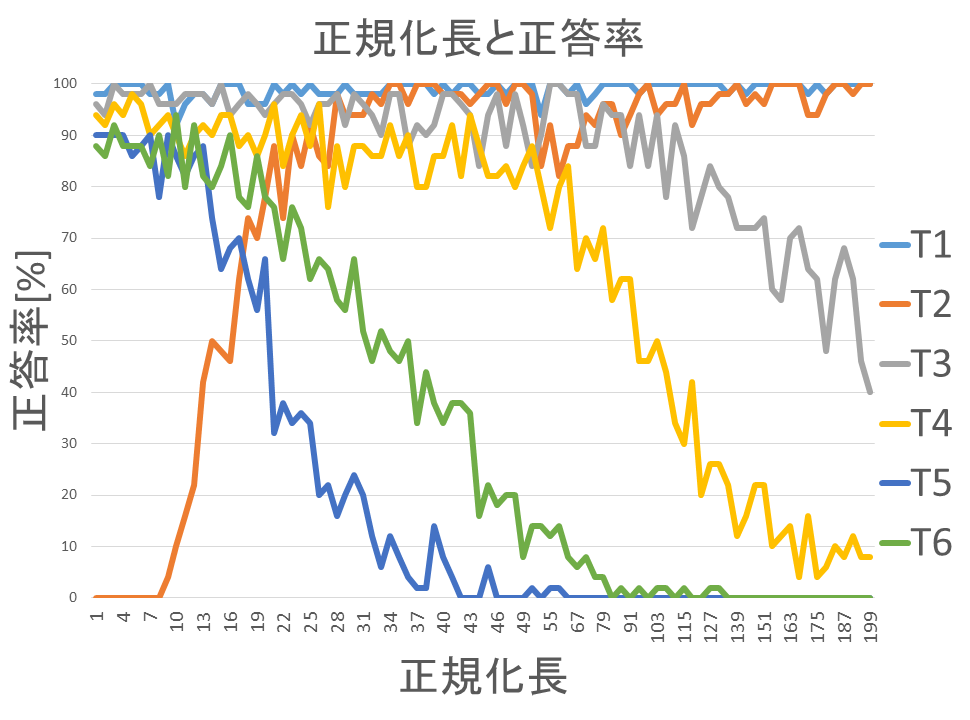
\includegraphics[width=7.5cm]{chart11_a.png} \\ %TeXの基本として, \\ で緊急改行ができる.(今回の場合や行列などを除き,あまり使わない)
		\subcaption{全動作}
		\label{subfigure:unit_a}    
	\end{minipage}
	\begin{minipage}[t]{.49\textwidth}
		\centering
		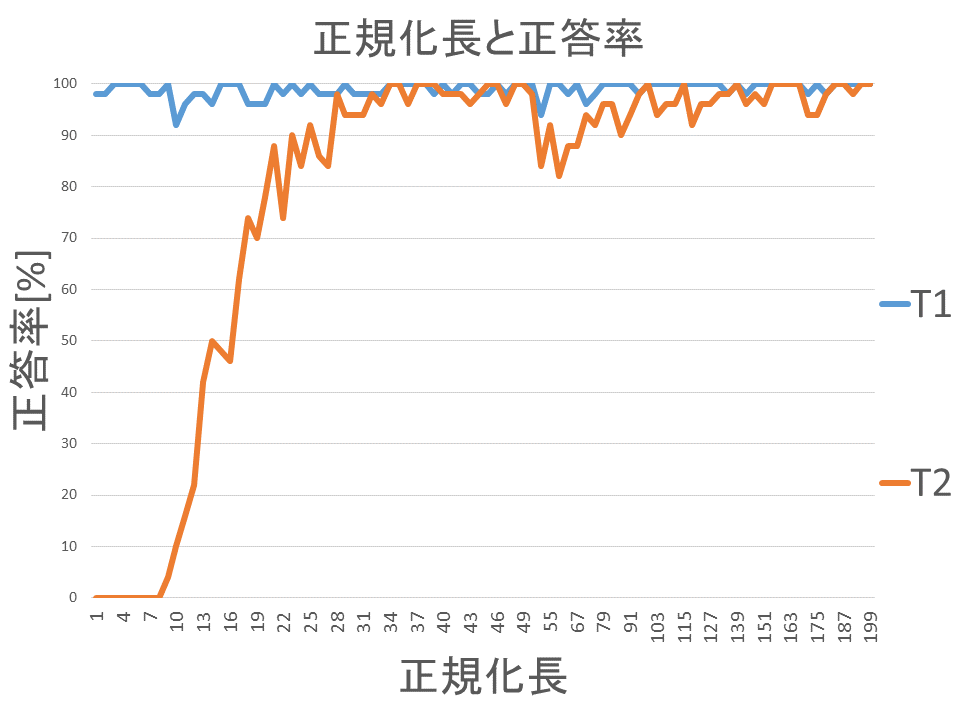
\includegraphics[width=7.5cm]{chart11_b.png} \\ %TeXの基本として, \\ で緊急改行ができる.(今回の場合や行列などを除き,あまり使わない)
		\subcaption{$T_{1}$,$T_{2}$}
		\label{subfigure:unit_b}
	\end{minipage}
	\begin{minipage}[t]{.49\textwidth}
		\centering
		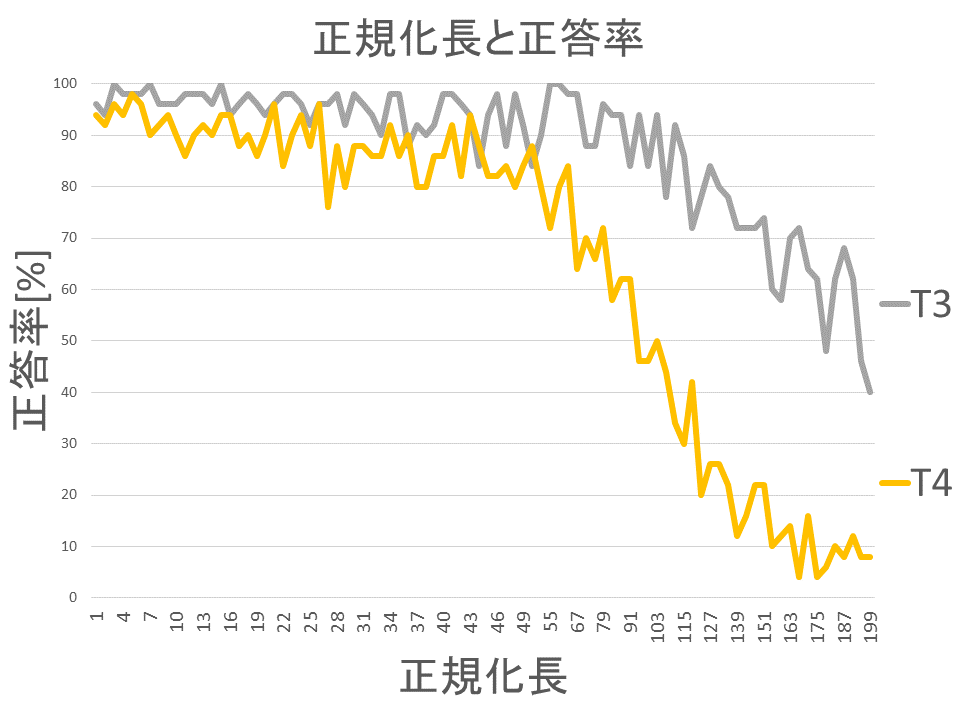
\includegraphics[width=7.5cm]{chart11_c.png} \\ %TeXの基本として, \\ で緊急改行ができる.(今回の場合や行列などを除き,あまり使わない)
		\subcaption{$T_{3}$,$T_{4}$}
		\label{subfigure:unit_c}
	\end{minipage}
	\begin{minipage}[t]{.49\textwidth}
		\centering
		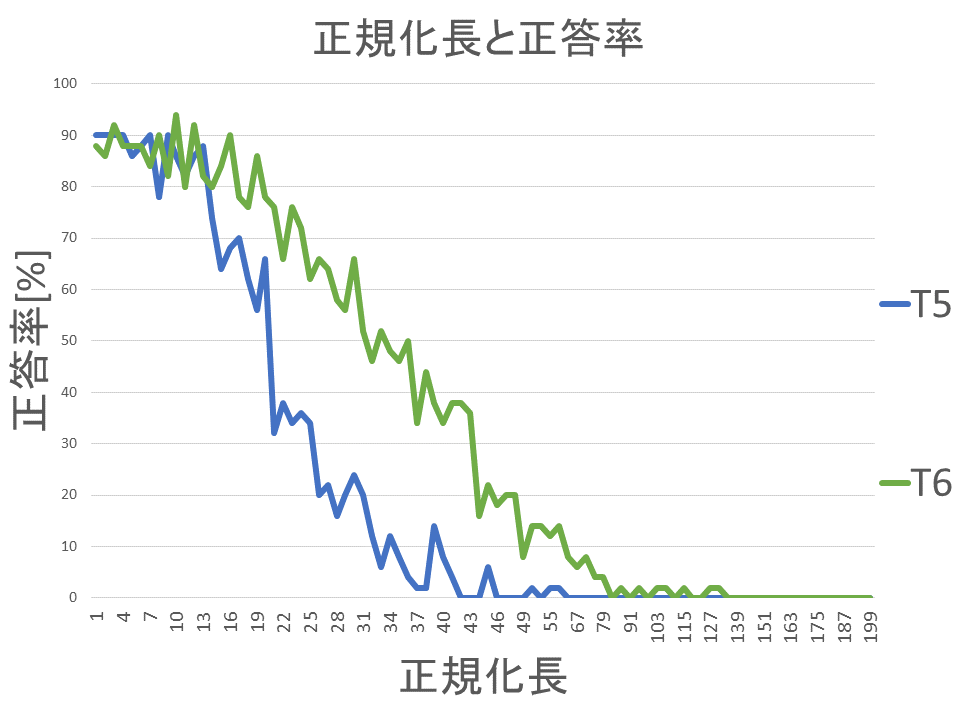
\includegraphics[width=7.5cm]{chart11_d.png} \\ %TeXの基本として, \\ で緊急改行ができる.(今回の場合や行列などを除き,あまり使わない)
		\subcaption{$T_{5}$,$T_{6}$}
		\label{subfigure:unit_d}
	\end{minipage}
	\caption{正規化長と正答率の関係のグラフ}
	\label{figure:success_rate_for_UNIT}
\end{figure}
%%%%%%%%%%%%%%%%%%%%%%%%%%%%%%%%%%%%%%%%%%%%%%%%%%%%%%%%%%%%%%%%%%%%%%%%%%%%%%%%%%%%%%%%%%%%%%%%%%%%%%%


\section{動作識別}

動作名が未知である例示動作を与え,それが既学習動作のうちいずれであるかを推定する実験を行った.
既学習動作はTable \ref{table:taskname_15}の6動作に,各動作に関して変位が等しく参照点を変えて生成した9動作を加えた計15動作とした.
各動作において教示動作として分散3のガウス誤差を持つ30データを生成し学習を行った.例示動作は動作再現実験と同様の6動作を使用し,各動作分散10のガウス誤差を持つ100データを生成してテストを行った.Table \ref{table:result}に各例示動作の識別正答率を示す.
Table \ref{table:result}より,学習済みの動作に関して例示動作の識別が適切に行えていることがわかる.また,誤識別が生じた初期環境と例示動作の例をFig.\ref{figure:failure}に示す.Fig.\ref{subfigure:failure1}は赤を橙に近づける例示動作だが,赤を緑から遠ざける動作だと誤って識別されている.誤識別が生じた例示動作に関しては,ほとんどがこのように人間にとっても適切な動作が判別し難いものであった.

\begin{table}[h]
	\caption{動作識別の正答率}
	\label{table:result}
	\centering
  	\begin{tabular}{|l|l|} \hline
    	動作名 & 正答率\\ \hline
   	赤を中央に移動する 		& 0.96
    	\\
    	赤を青の右に移動する 		& 0.98
    	\\
    	赤を橙に近づける 			& 0.97
    	\\
    	赤を緑から遠ざける 			& 0.97
    	\\
    	等間隔に赤,黄,青と並べる 	& 1.00
    	\\
    	時計回りに赤,緑,青と並べる 	& 0.96
    	\\ \hline
  	\end{tabular}
\end{table}

%%%%%%%%%%%%%%%%%%%%%%%%%%%%%%%%%%%%%%%%%%%%%%%%%%%%%%%%%%%%%%%%%%%%%%%%%%%%%%%%%%%%%%%%%%%%%%%%%%%%%%%
\begin{figure}[h]
	\centering
	\begin{minipage}[t]{.47\textwidth}
		\centering
		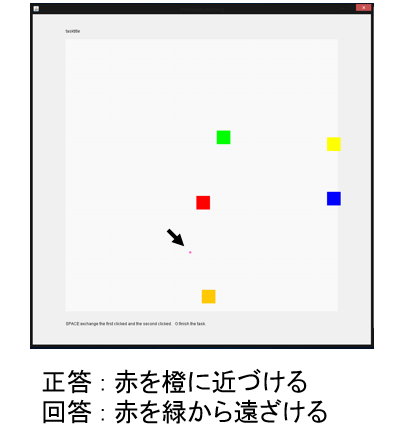
\includegraphics[width=7cm]{figure4_a.png} \\ %TeXの基本として, \\ で緊急改行ができる.(今回の場合や行列などを除き,あまり使わない)
		\subcaption{誤識別の例1}
		\label{subfigure:failure1}    
	\end{minipage}
	\begin{minipage}[t]{.47\textwidth}
		\centering
		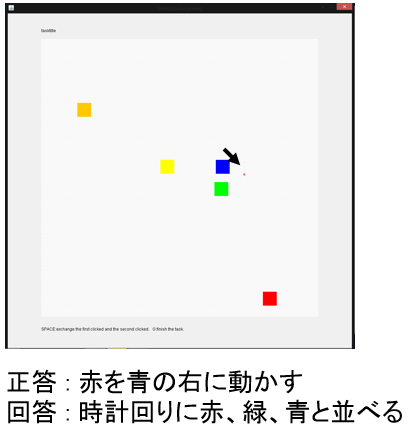
\includegraphics[width=7cm]{figure4_b.png} \\ %TeXの基本として, \\ で緊急改行ができる.(今回の場合や行列などを除き,あまり使わない)
		\subcaption{誤識別の例2}
		\label{subfigure:failure2}
	\end{minipage}
	\caption{誤識別の例}
	\label{figure:failure}
\end{figure}
%%%%%%%%%%%%%%%%%%%%%%%%%%%%%%%%%%%%%%%%%%%%%%%%%%%%%%%%%%%%%%%%%%%%%%%%%%%%%%%%%%%%%%%%%%%%%%%%%%%%%%%
